\begin{enumerate}[label=\thesection.\arabic*.,ref=\thesection.\theenumi]
\numberwithin{equation}{enumi}

\item
Consider a unity feedback system as shown in the figure,shown with an integral compensator k/s and open-loop transfer function
\begin{align}
G(s) = \frac{1}{s^2+3s+2}
\end{align}
where k greater than 0. The positive value of k for which there are two poles of unity feedback system on j${\omega}$ axis is equal to-----(rounded off to two decimal places)
%\centering
%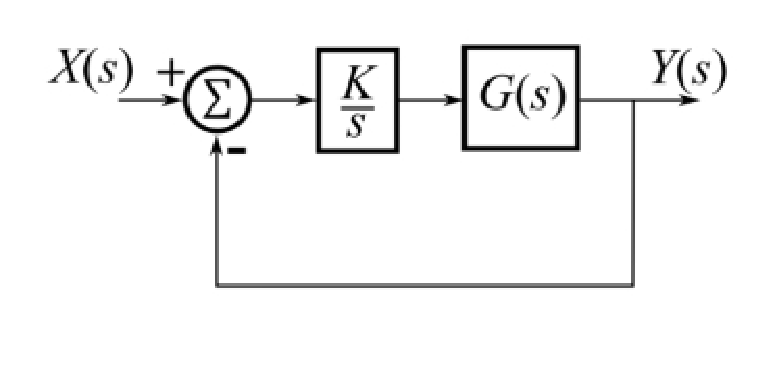
\includegraphics[width=\columnwidth]{ee18btech11005.eps}
\begin{figure}
\centering
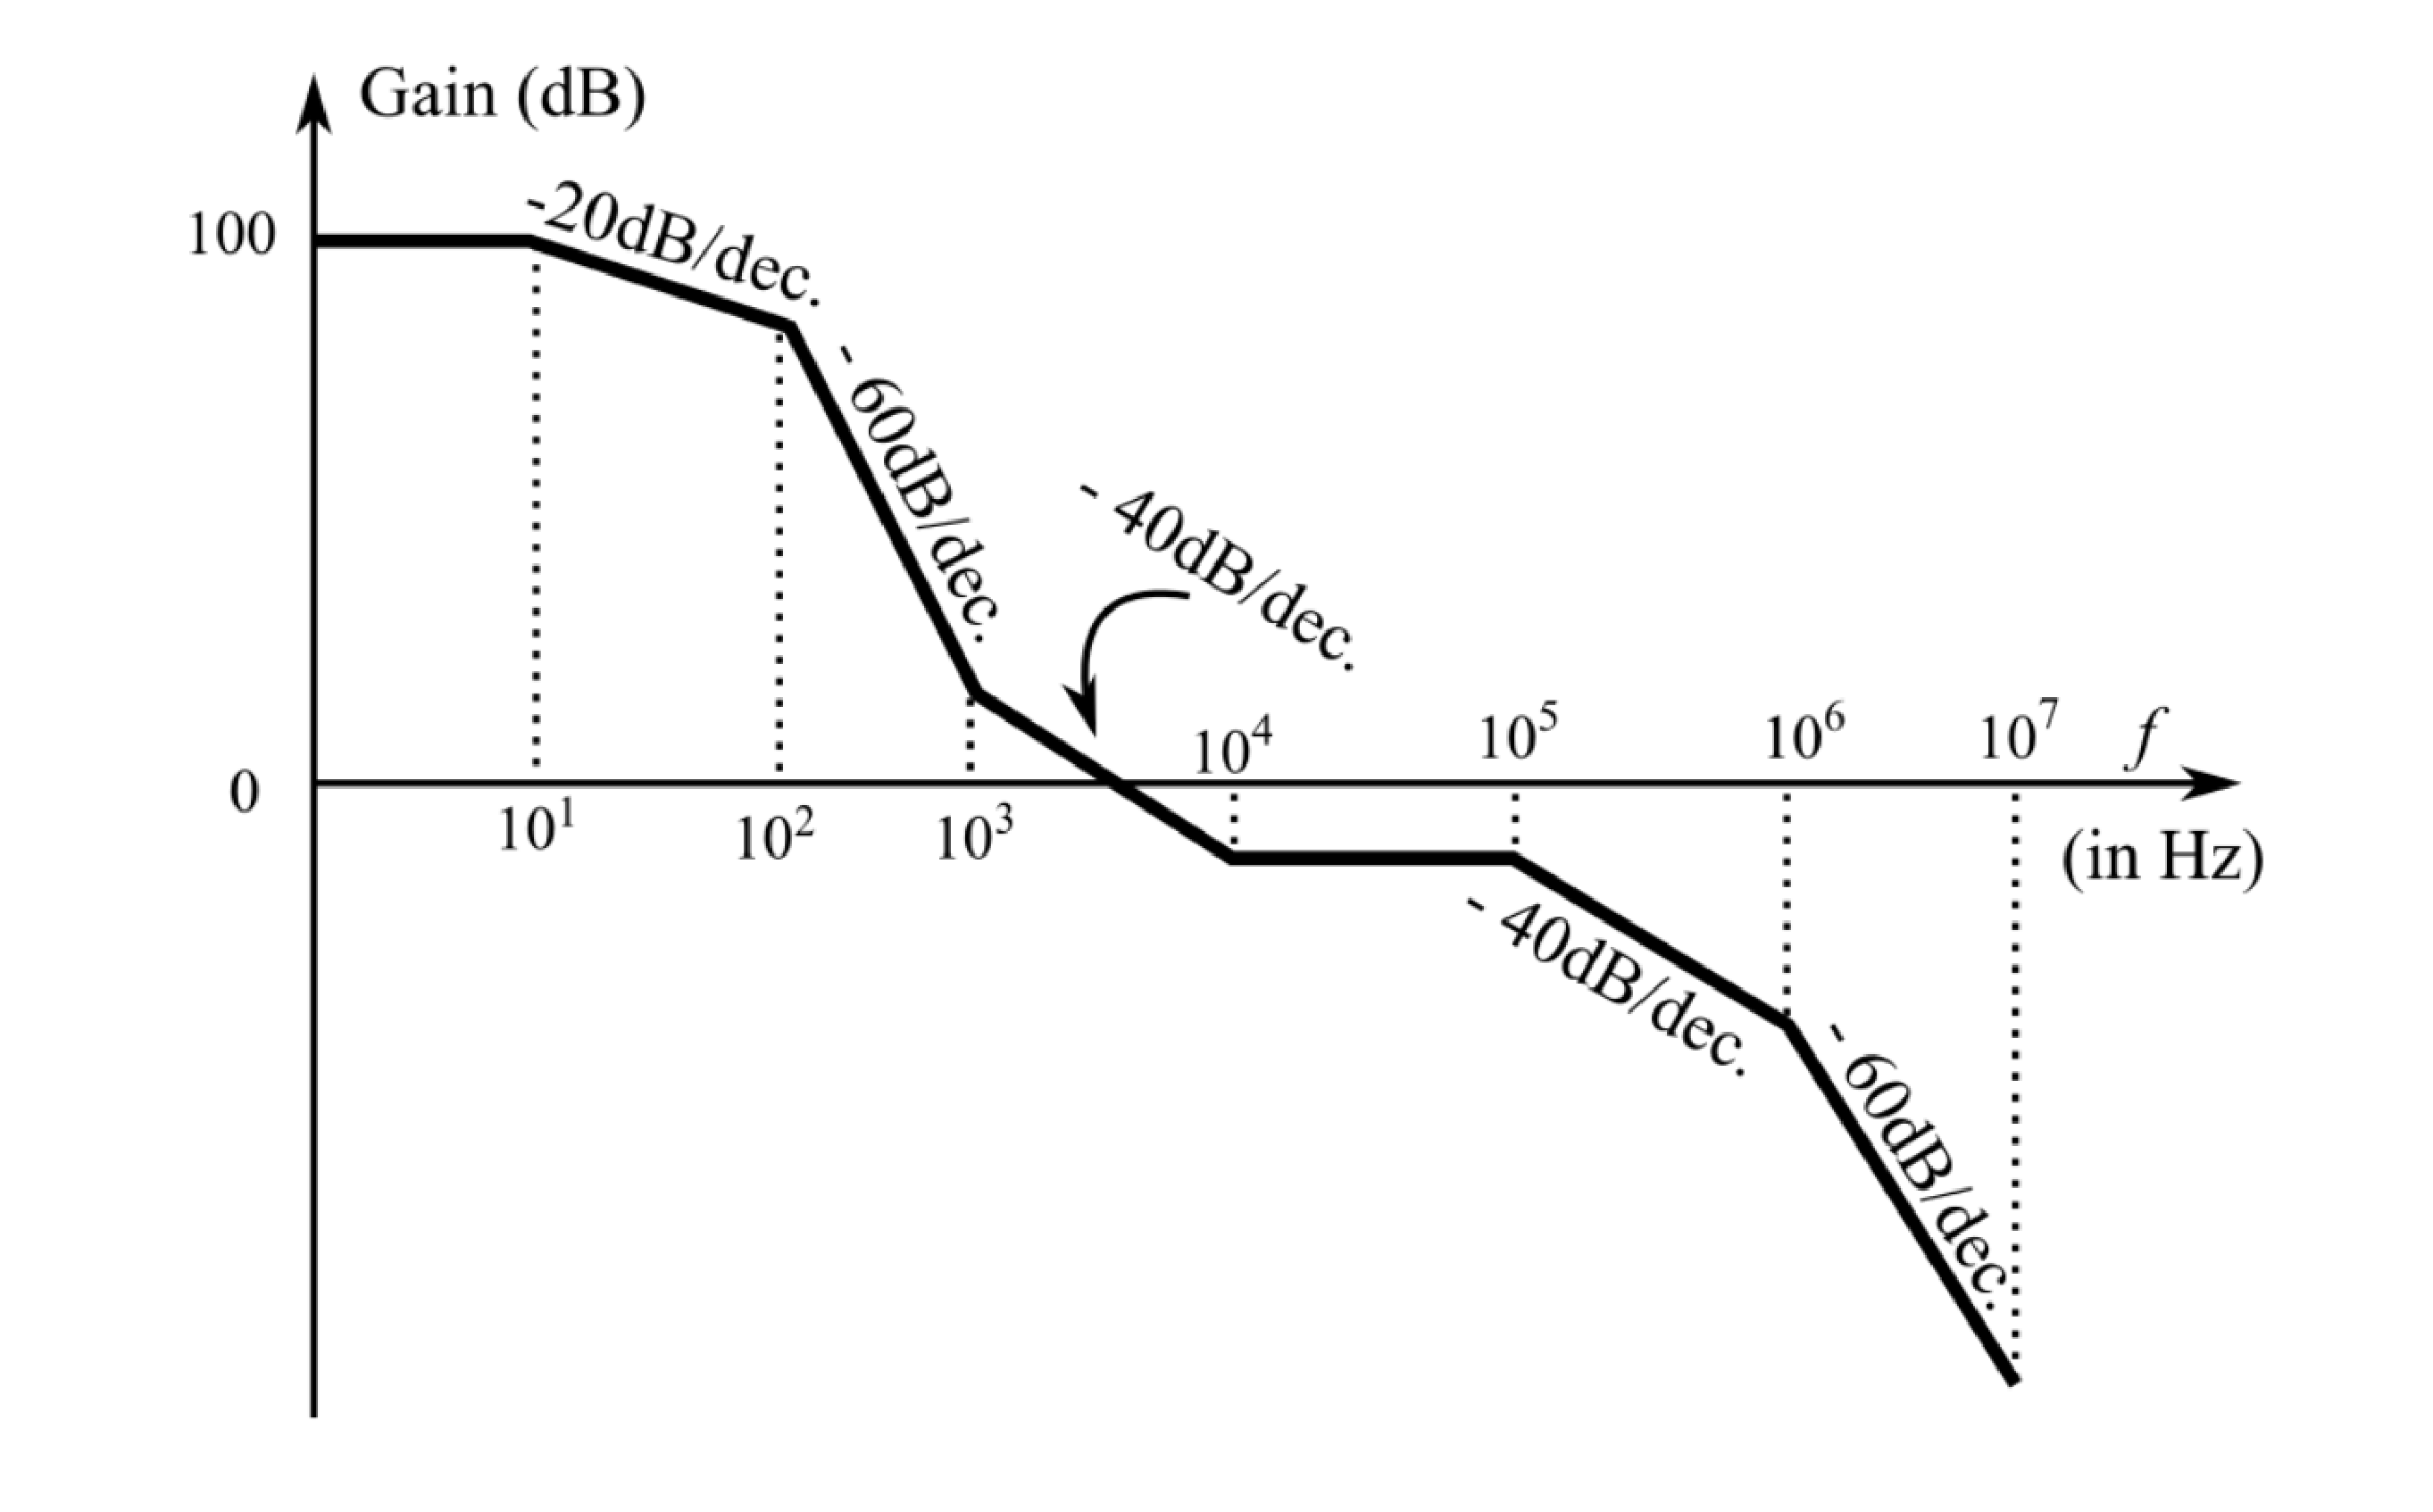
\includegraphics[width=\columnwidth]{figure.eps}
\end{figure}
\solution The transfer function for negative feedback is given by
\begin{align}
\frac{Y(s)}{X(s)} &= \frac{G(s)}{1+G(s)H(s)}
\end{align}
where H(s) = 1 for unity feedback system
and G(s) is net forward open loop gain
\begin{align}
G(s) &=  \sbrak{\frac{1}{s^2+3s+2}}\sbrak{\frac{k}{s}}
&= \frac{k}{s^3+3s^2+2s}
\end{align}
Characteristic equation is..,
\begin{align}
 1 + G(s)H(s) = 0 \label{eq:sec_order_op}
\\
=> 1 + \sbrak{\frac{k}{s^3+3s^2+2s}} = 0
\\
=> s^3+3s^2+2s+k = 0
\end{align}
The Routh hurwitz criterion:-
This criterion is based on arranging the coefficients of characteristic equation into an array called Routh array.
For any characteristic equation q(s),
\begin{multline}
q(s) = a_0s^n+a_1s^{n-1}+.....+a_{n-1}s+a_n = 0
\end{multline}
Routh array can be constructed as follows..,
 
\myvec{s^n\\s^{n-1}\\s^{n-2} \\ \vdots}
 \myvec{a_0 & a_2 & a_4 & \cdots \\
a_1 & a_3 & a_5 & \cdots  \\
b_1 & b_2 & b_3 & \cdots \\
\vdots & \vdots & \vdots & \ddots &\vdots 
 \cdots \\}
 \\
 where
 \begin{align}
 b_1 =\frac{ a_1a_2-a_0a_3}{a_1}  
 \\
 b_2 =\frac{ a_1a_4-a_0a_5}{a_1} 
 \\
 c_1=\frac{ b_1a_3-a_1b_2}{b_1} 
\\
 c_2=\frac{ b_1a_5-a_1b_3}{b_1}  
\end{align}
For poles to lie on imaginary axis any one entire row of hurwitz matrix should be zero.
Constructing the routh array for the characteristic equation obtained in equation(\ref{eq:sec_order_op})
\begin{align}
 s^3+3s^2+2s+k = 0
\end{align}
%
\begin{align}
\myvec{s^3\\s^2\\s^1 \\ s^0}
\myvec{1 & 2 \\ 3 & k \\  \frac{6-k}{3} & 0\\ k & 0} \label{eq:sec_order_op_1}
\end{align}
For poles on j$\omega$ axis any one of the row should be zero.
\begin{align}
\frac{6-k}{3} = 0 \hspace{5pt} or\hspace{5pt} k = 0
\end{align}
But given k greater than 0 ...
\begin{align}
   6-k = 0\\
   k = 6
\end{align}
\item Repeat the above using the determinant method.
\solution
Determinent method:
\myvec{a_0 & a_2 & a_4 & \cdots \\
a_1 & a_3 & a_5 & \cdots  \\
 0 & a_0 & a_2\cdots \\
 0 & a_1 & a_3 \cdots\\
\vdots & \vdots & \vdots & \ddots &\vdots 
\cdots \\}
\begin{align}
D1 &= |a_0|
\\
D2 &= \begin{vmatrix}
a_0 & a_2 \\ a_1 & a_3 \end{vmatrix}
\\
D3 &=\begin{vmatrix}
a_0 & a_2 & a_4 \\ a_1 & a_3 & a_5 \\ 0 & a_0 & a_2 \end{vmatrix}
\end{align}
and so on...
If atleast any one of the Determinents are zero then the poles lie on imaginary axes.
So,For the given question the routh array is obtained from equation(\ref{eq:sec_order_op})
\begin{align}
D1 &= 1
\\
D2 &= \begin{vmatrix}
1 & 2 \\ 3 & k \end{vmatrix} 
&= k-6
\\
D3 &=\begin{vmatrix}
1 & 2 & 0 \\ 3 & k & 0 \\ 0 & 1 & 2 \end{vmatrix}
&=2k-12
\end{align}
D2 = k-6 =0 for the poles to lie on imaginary axis
\begin{align}
   k-6 = 0\\
   k = 6
\end{align}
\item Verify your answer using a python code for both the determinant method as well as the tabular method.
\solution 
The following code 
%
\begin{lstlisting}
codes/ee18btech11005/routhhurwitztabular.py
\end{lstlisting}
\end{enumerate}
